% Šablona pro maturitní práci Gymnázia Jírovcova 8, České Budějovice
% Autoři šablony: Jonáš Havelka, Michal Kočer, Daniel Sýkora
% Typ dokumentu: report
% veškeré úpravy v soubor MP.sty (styl maturitní práce)
\documentclass[12pt]{report}
% %%%%%%%%%%%%%%%%%%%%%%%%%%%%%%%%%%%%%%%%%%%%%%%%%%%%%%%
\usepackage{MP}						  % Import stylu maturitní práce
\author{Kryštof Maxera}                  % AUTOR PRÁCE
\title{Konstrukce dronu}    % NÁZEV PRÁCE
\date{14. února 2025}                 % DATUM ODEVZDÁNÍ PRÁCE
\vedouci{Dr.rer.nat Michal Kočer} % VEDOUCÍ PRÁCE
\place{V Českých Budějovicích}
\skolnirok{2024/2025}                  % ŠKOLNí ROK
\logo{
\includegraphics[scale=1.25]{GJ8_logotyp}} %Logo školy
%%%%%%%%%%%%%%%%%%%%%%%%%%%%%%%%%%%%%%%%%%%%%%%%%%%%%%%%%%%%%%%%%%%
\begin{document} %%%%%%% začátek dokumentu
%%%%%%%%%%%%%%%%%%%%%%%%%%%%  Titulní stránka + úvodní povinné stránky
\pagenumbering{roman}                   % číslování stránek římskými číslicemi
	\mytitlepage						% Vygenerování titulní strany
	
	\prohlaseni{
		Prohlašuji, že jsem tuto práci vypracoval samostatně s vyznačením všech použitých pramenů.
	}	
	
	\abstrakt{
		\lipsum[1]						% Abstrakt 
	}{
		\lipsum[1]						% Klíčová slova
	}
	
	\podekovani{
		\lipsum[2]						% Poděkování
	}
	
   {\tableofcontents\newpage}			% Obsah
	
%%%%%%%%%%%%%%%%%%%%%%%%%%%% VLASTNÍ PRÁCE
\addtocounter{page}{1}		% Posunutí countru stránek
\pagenumbering{arabic}		% Číslování stránek arabskými číslicemi
\chapter*{Úvod}     % úvod práce 
	
\lipsum[1]	
	
%%%%%%%%%%%%%% TEORETICKÁ ČÁST %%%%%%%%%%%%%%%%%%	
\part{Úvod do světa dronů}  % název teoretické části (nenechávejte Teoretická část)
	
\chapter[Definice a charakteristika dronů]{Definice a charakteristika dronů}

Dron je definován jako zařízení nebo stroj schopný vykonávat úkoly bez nutnosti přímé fyzické přítomnosti člověka. Tato zařízení lze rozdělit do dvou základních kategorií.

První kategorii tvoří plně autonomní roboti, u jichž je přítomnost člověka vyžadována primárně z kontrolních a bezpečnostních důvodu. Pilot nebo operátor zde většinou nezasahuje do aktivního řízení, ale v případě potřeby může převzít kontrolu. Typickým příkladem jsou autonomní bezpilotní letadla s možností vzdáleného ovládání nebo samořízené motorové vozidlo, které ke svému provozu nepotřebuje řidiče přítomného ve vozidle.

Druhá kategorie je pro veřejnost známější. Ta je také nazývána drony, přestože její součástí jsou dálkově ovládaná zařízení, která nejsou plně autonomní. Do této skupiny patří široce známé kvadrokoptéry a další multikoptéry, stejně jako autíčka na dálkové ovládání.

Důvodem časté záměny těchto dvou kategorií je překrývání některých funkcí, neboť i dálkově ovládané kvadrokoptéry využívají automatické systémy, například pro samovyvažování, které jsou nezbytné pro jejich stabilní let.\\

Drony lze obecně rozdělit do několika hlavních skupin na základě prostředí, ve kterém operují:
\begin{itemize}
	\item \textbf{Bezpilotní letadla} (UAVs - Unmanned Aerial Vehicles)
	\item \textbf{Bezpilotní pozemní vozidla} (UGV - Unmanned Ground Vehicle)
	\item \textbf{Hladinové plavidla bez posádky} (USV - Unmanned Surface Vehicle)
	\item \textbf{Dálkově ovládané podvodní vozidla} (ROUV - Remotely Operated Underwater Vehicles)
	\item \textbf{Bezpilotní kosmické lodě} (Uncrewed spacecraft)
\end{itemize}

Přestože označení dron lze použít pro širokou škálu zařízeních, pro širokou veřejnost je toto slovo primárně spjaté s dálkově ovládanými bezpilotními letadly. Samo o sobě však toto označení není chybné. V této práci se zaměřujeme na konstrukci kvadrokoptéry, která spadá do kategorie bezpilotních letadel. O té práce pojednává podrobněji. \cite{mainbook}

\section{Bezpilotní letadla}

Bezpilotní letadlo je definováno jako zařízení určené k provozu ve vzdušném prostředí, které je buď řízeno dálkově operátorem, nebo schopno autonomního letu díky integrovanému softwaru a palubním senzorům. 

Tato zařízení využívají pokročilé technologie pro navigaci, stabilizaci, komunikaci a sběr dat, přičemž jejich provozní komponenty se liší v závislosti na specifickém účelu použití. Obecně však tato zařízení zahrnují senzory nezbytné pro stabilizaci letu, jako je gyroskop a akcelerometr, spolu se senzory či moduly umožňujícími komunikaci. Komunikační technologie obvykle zahrnují přenos dat prostřednictvím rádiových vln, Wi-Fi, nebo mobilních sítí.

Tato zařízení lze dále klasifikovat na základě specifických parametrů, jako je typ konstrukce křídla, hmotnost, zdroj napájení či funkční zaměření.\\

Při klasifikaci na základě typu konstrukce křídla lze bezpilotní letadla rozdělit do dvou hlavních skupin:
\begin{itemize}
	\item Rotorová letadla - zahrnující jednorotorové a vícerotorové varianty, jako jsou trikoptéry, kvadrokoptéry, hexakoptéry a oktokoptéry.
	\item Letadla s pevnými křídly - zahrnují drony, které vyžadují pohyb vpřed k generování vztlaku pomocí křídel. Patří sem také hybridní drony s vertikálním vzletem a přistáním, jež nevyžadují přistávací dráhu.
\end{itemize}

Zařazení na základě zdroje napájení:
\begin{itemize}
	\item Bateriový pohon - nejčastěji lithium-polymerové (Li-Po) nebo lithium-iontové (Li-Ion) baterie
	\item Benzínový pohon - spalovací motor poháněný benzínem
	\item Vodíkový pohon - napájení je zajištěno vodíkovými palivovými články, které generují elektrickou energii chemickou reakcí
	\item Solární pohon - solární panely umístěné na povrchu dronu zajišťují nepřetržité nabíjení během letu
\end{itemize}

Zařazení na základě nejběžnějších funkčních kategorií:
\begin{itemize}
	\item rekreační využití
	\item letecká fotografie a videografie
	\item pátrací a záchranné operace
	\item vojenský průmysl
	\item stavební průmysl, monitorování a měření
	\item zemědělství
	\item dopravní a logistické služby
\end{itemize}

Tato skupina zařízení byla po dlouhou dobu spojována především s vojenským průmyslem. V současnosti však díky široké škále aplikací nacházejí stále větší uplatnění i v civilních oblastech, jako je průmysl, zemědělství nebo vědecký výzkum. Díky klesajícím cenám se osobní kvadrokoptéry stávají stále populárnějšími také pro rekreační účely. \cite{mainbook} \cite{whatisadrone}\\

\section{Bezpilotní pozemní vozidla}
Jedná se o pozemní vozidla bez potřebné fyzické přítomnosti člověka. Ve srovnání se vzdušnými bezpilotními drony jsou mnohem jednodušší na konstrukci, protože nevyžadují překonávání fyzikálních zákonů spojených s letem. Tato vlastnost přispívá k jejich širokému využití napříč různými sektory. Lze je nalézt například v zemědělství jako samosklízecí traktory, v oblasti samořídících dopravních prostředků, v těžebním průmyslu, v automatizovaných skladech s roboty pro transport zboží nebo v úklidovém sektoru, kde se využívají autonomní vysavače. Své uplatnění nacházejí také ve vojenském sektoru. \cite{mainbook}

\section{Hladinové plavidla bez posádky}
Plavidla pohybující se po mořské nebo sladkovodní hladině. Často jsou využívána pro těžební operace na moři, vědecký výzkum či monitorování vodních ekosystémů. Nelze opomenout jejich vojenské využití. Tato zařízení používají pro komunikaci obdobné technologie jako bezpilotní letadla. \cite{mainbook}

\section{Dálkově ovládané podvodní vozidla}
Podvodní zařízení, určená převážně pro průzkumné a vědecké účely, představují klíčový nástroj pro studium mořského prostředí. Jejich fungování se však výrazně liší od ostatních autonomních systémů, a to kvůli technickým výzvám spojených s provozem ve velkých hloubkách. V těchto podmínkách je použití rádiových vln pro komunikaci téměř nemožné kvůli jejich omezené prostupnosti vodou. Namísto bezdrátové komunikace jsou proto tato zařízení často spojena s mateřskou lodí nebo ponorkou pomocí robustního kabelu, který slouží nejen jako přenosové médium pro data, ale i jako zdroj energie. \cite{mainbook}

\section{Bezpilotní kosmické lodě}
Vesmír představuje ideální prostředí pro využití dronů, neboť je pro lidskou přítomnost extrémně nehostinný. Vesmírné drony nabízejí méně rizikové řešení pro dosažení různých cílů bez nutnosti návratu zařízení zpět na Zemi. Jejich využití zahrnuje kosmický prostor, kde slouží k prozkoumávání vzdálených objektů, povrchy nehostinných planet, kde fungují jako rovery, a oběžnou dráhu Země, kde podporují fungování klíčových technologií, jako je například GPS. \cite{mainbook}\\

Využití všech těchto typů dronů má společnou vlastnost. Jejich využití je na místech, kde lze pracovní sílu člověka nahradit automatickým zařízením nebo místech, které jsou příliš riskantní pro přítomnost člověka. Jejich nasazení se neustále rozšiřuje a lze bez pochybností předpokládat, že v budoucnu bude jejich význam dále narůstat.

\chapter[Anatomie multikoptéry]{Anatomie multikoptéry}
Každá multikoptéra, ať už profesionálně vyrobená nebo sestavená v domácích podmínkách, se liší svým konstrukčním hardwarem. Nicméně většinu těchto zařízení spojuje použití podobných klíčových komponent. Tato kapitola se zaměřuje na podrobný popis nejběžnějších součástek, které byly využity při konstrukci kvadrokoptéry v praktické části práce.

\section{Rám}
Rám dronu tvoří základní konstrukční prvek, který drží všechny komponenty pohromadě. Typ rámu použitý u dronu má zásadní vliv na jeho celkové vlastnosti. Klíčovým aspektem při výběru a návrhu rámu je nalezení optimálního poměru mezi hmotností, velikostí a pevností, aby konstrukce byla co nejvíce odolná vůči nárazům a pádům, zároveň však nezvyšovala zbytečně hmotnost zařízení. Tento vyvážený design hraje významnou roli ve stabilitě, ovladatelnosti a životnosti dronu.

\subsection{Tvar}
První klíčovou vlastností rámu, na kterou je třeba se zaměřit, je jeho tvar. Konstrukce rámu musí odpovídat počtu vrtulí, což vyžaduje adekvátní počet ramen. Například trikoptéry disponují třemi rameny, hexakoptéry šesti, zatímco nejběžnější kvadrokoptéry mají čtyři ramena.Důležitým konstrukčním aspektem je také úhel mezi jednotlivými rameny, který ovlivňuje nejen stabilitu a letové vlastnosti dronu, ale také případné zorné pole připevněné kamery.

\subsection{Materiál}
Výběr materiálu rámu výrazně ovlivňuje dvě klíčové vlastnosti dronu: hmotnost a odolnost. Existuje široká škála materiálů vhodných pro konstrukci rámu. Základním kritériem je dostatečná pevnost materiálu, která umožňuje jeho použití jako nosné struktury. Některé materiály poskytují výrazné výhody, díky nimž jsou preferovány.\\

Nejčastěji používané materiály zahrnují:
\begin{itemize}
	\item Uhlíkové vlákno - vynikající pevnost a nízká hmotnost, vysoká cena, pro profesionální konstrukce
	\item Dřevo - snadná dostupnost, výborná tvarovatelnost, vhodné pro malé multikoptéry
	\item Hliník - vysoká pevnost a odolnost, nízká cena, vysoká hmotnost
	\item Pěna - převážně u malých dronů díky své nízké hmotnosti, omezená stabilita
	\item Plast - levný, lehký a snadno tvarovatelný materiál, možné použití 3D tisku
\end{itemize}

\subsection{Velikost}
V neposlední řadě je potřeba zvolit správnou velikost dronu.  Obecně platí, že s rostoucí velikostí dronu se zvyšuje jeho hmotnost, ale zároveň i stabilita. Volba optimální velikosti závisí na požadovaných letových vlastnostech a plánovaném zatížení dronu.

\section{Motory}
\lipsum[1]

\section{Vrtule}

\lipsum[1]

\section{ESPs}

\lipsum[2]

\section{Flight controller}
\lipsum[3]

\section{Raspberry Pi Pico}


\section{Baterie}

\section{Airframe}


\lipsum[3]

\chapter{Fyzika letu dronu}

\lipsum[1]

%%%%%%%%%%%%%% PRAKTICKÁ ČÁST %%%%%%%%%%%%%%%%%%	
\part{Konstrukce kvadrokoptéry} % název praktické části (nenechávejte název Praktická část)

\chapter{Součástky}
\lipsum[1]	

\chapter{Průběh Konstrukce}

\lipsum[1]	

\section{Druhy dronů}
	Odkaz v závorkách: \parencite[see][page 900]{einstein}\\
	Odkaz: \cite{knuthwebsite}\\
	A odkaz pod čarou: \footcite[see][s. 42]{latexcompanion}\\
	Dobrý den, ahoj, \gls{atd}\\
	Praha, \gls{tj} hlavní město ČR
	



\chapter[Stručná historie dronů]{Stručná historie dronů}
%%% v obsahu se objeví jen to co je v hranatých závorkách
\begin{figure}
  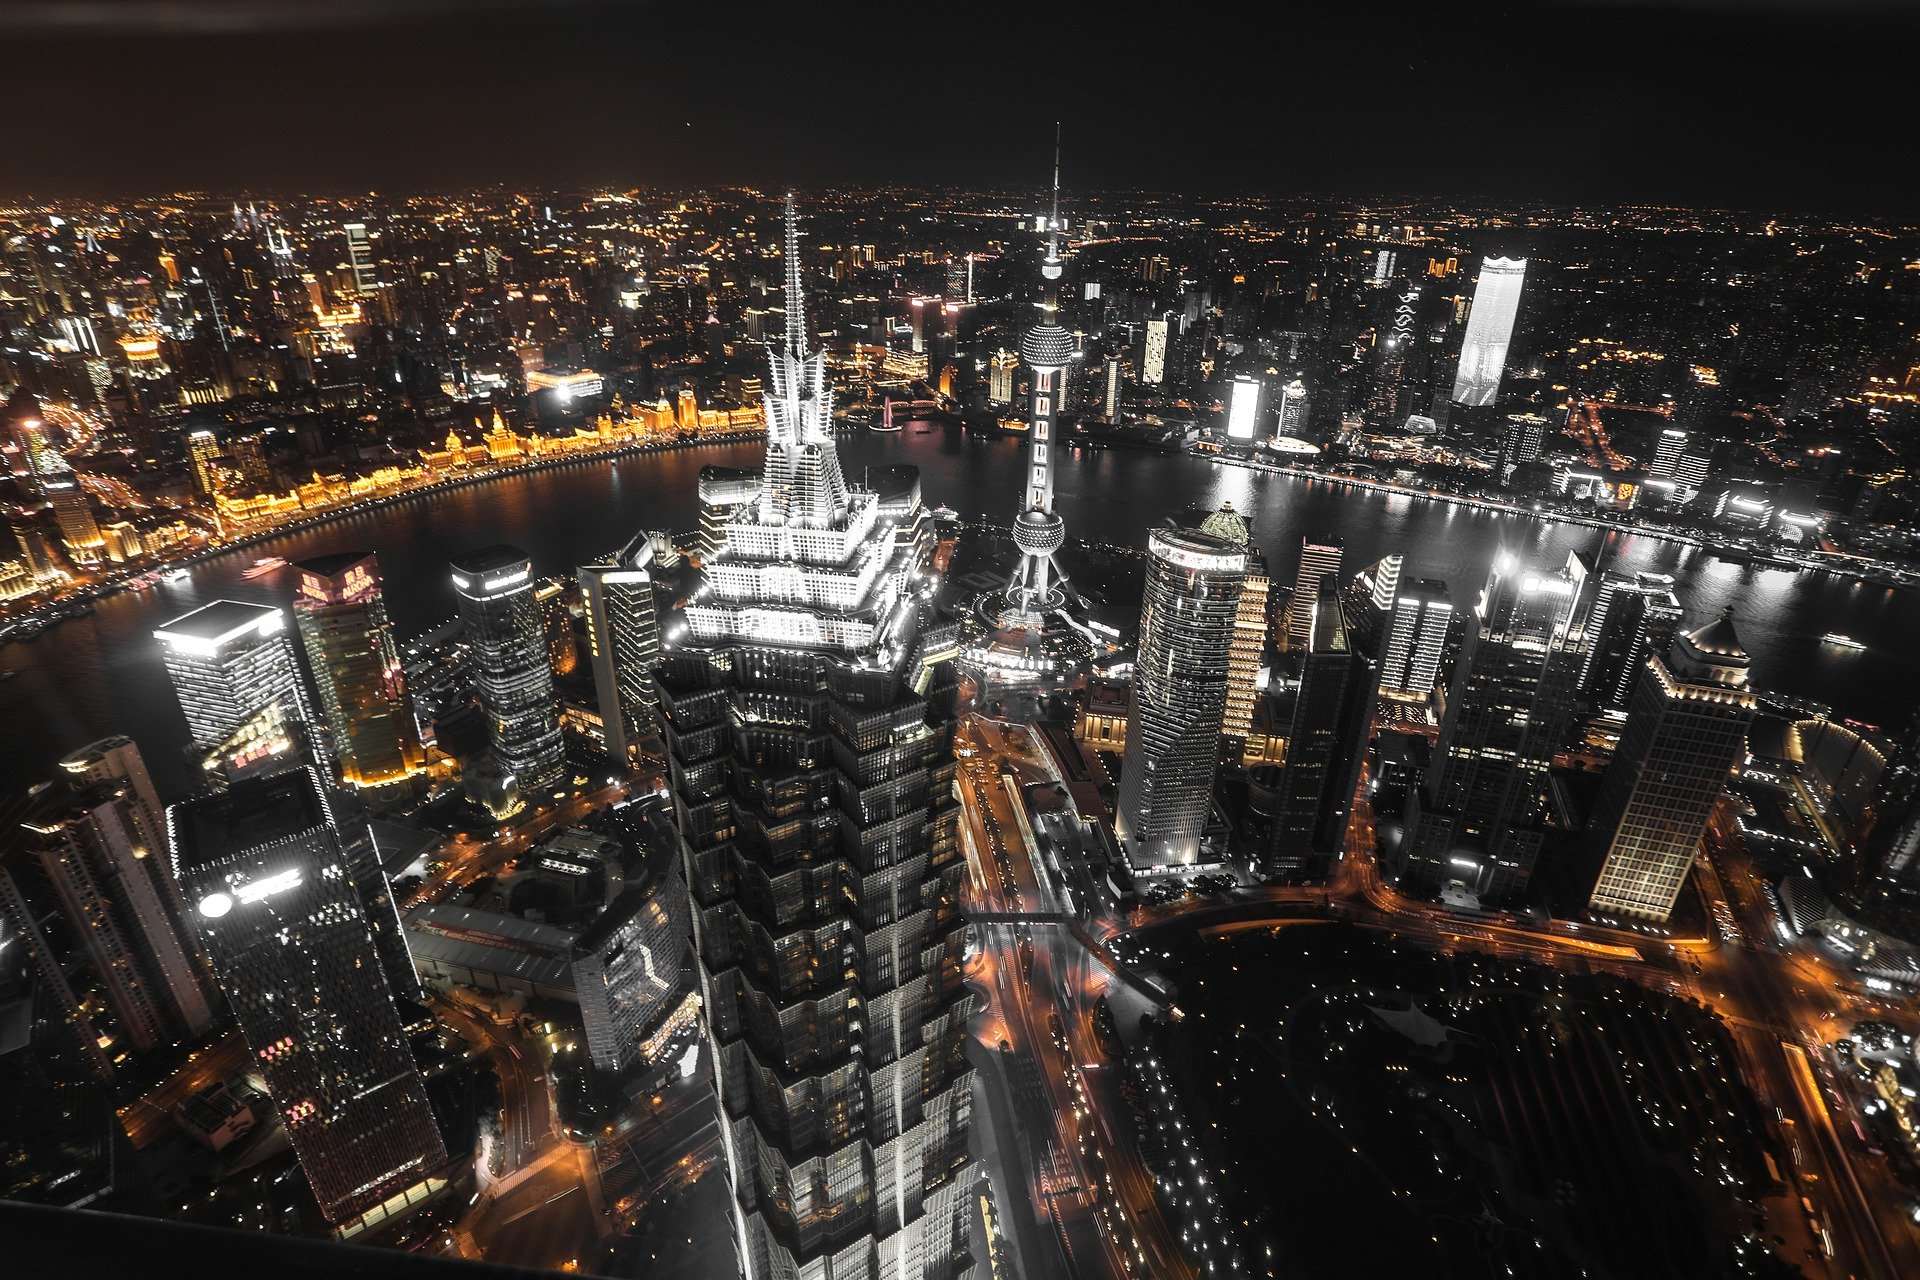
\includegraphics[width=\linewidth]{test.jpg}
  \caption{Testovací}
  \label{fig:test}
\end{figure}
Obrázek \ref{fig:test} ukazuje Shangai z Pixabay.\\
Tabulka \ref{tab:test2} ukazuje hádejte, co.
	
\lipsum[3]


Výpis programu \nameref{lst:hello_world}  naleznete ve výpise \ref{lst:hello_world}.

\begin{lstlisting}[title={Program hello.c}, caption={hello.c}, label={lst:hello_world}]
#include <stdio.h>
#define CISLO 10

int main(void) {
	int i = CISLO;

	print("Hello World!\n");
	print("%d", i);

	return (0);
}
\end{lstlisting}

\lipsum[1]	

\begin{lstlisting}[numbers=none, title={Příklad výstupního souboru}]
11.0524
5.5954
6.7996
13.8584
15.1357
Soucet: 52.4415
\end{lstlisting}

\chapter{Program}

\lipsum[1]

\chapter{Schéma zapojení}

\lipsum[1]

%%%%%%%%%%%%% ZÁVĚR
\chapter*{Závěr}
	
\lipsum[1]
	
\nocite{*}
\printbibliography					% Vytvoří seznam literatury
\addcontentsline{toc}{chapter}{Bibliografie}
\printglossary[title={Zkratky}]		% Vytvoří seznam zkratek
\listoffigures						% Vytvoří seznam obrázků
\listoftables						% Vytvoří seznam tabulek

%%%%%%%%%%%%% PŘÍLOHY - APPENDIX 	
\begin{appendices}
	\chapter{Fotografie zkonstruované kvadrokoptéry}	
	\lipsum[1]
    	%\pitem{Fotky z pokusů}
    	%\eitem{Vlastní program}
    	%\eitem{Dokumentace}
    	%\eitem{Testovací data}
	\chapter{Kód programu Raspberry Pi Pico}  
\end{appendices}
%%%%%%%%%%%%%%%
\end{document}
%%%%%%%%%%%%%%%%%%%% KONEC %%%%%%%%%%%%%%%%%%%%%%%%%